\documentclass[11pt, letterpaper]{memoir}
\usepackage{HomeworkStyle}

\begin{document}
	\begin{center}
		{\large	Quiz 12.3 -- Vapor Pressure and Phase Diagrams}
	\end{center}
	{\large Name: \rule[-1mm]{4in}{.1pt} 
	
	\begin{center}	
	All questions will refer to the phase diagram for an unknown substance shown below
	\end{center}
	
	\noindent
	\begin{minipage}[T]{0.49\textwidth}
		\subsection*{Question 1}
		On the diagram, label the regions which represent each phase (solid, liquid, and gas)
		
		\subsection*{Question 2}
		Estimate the normal boiling temperature
		
		\hspace{1em}
		\subsection*{Question 3}
		Is the liquid or solid phase more dense?
		
	\end{minipage} \hspace{1em}
	\begin{minipage}[T]{0.49\textwidth}
		\includegraphics[width=\textwidth]{Phase_Diagram}
	\end{minipage}

	\vspace{1em}
	\subsection*{Question 4}
	Estimate the temperature and pressure at the triple point and the critical point
	
	\vspace{2em}
	\subsection*{Question 5}
	Use your estimates to calculate $\Delta H_{vap}$
	
	\vspace{6em}
	\subsection*{Question 6}
	Use the normal boiling point and your estimate of $\Delta H_{vap}$ to predict what the vapor pressure \emph{would be} at $120~^\circ C$, if there were no critical point
	
	
	\newpage
	\pagestyle{empty}
	\addtocounter{page}{-1}
	\section*{\emph{Птичка (A Little Bird)}}
	\paragraph{By Александр Сергеевич Пушкин (Alexander Sergeyevich Pushkin)}~
	
	\begin{verse}
		В чужбине свято наблюдаю\\
		Родной обычай старины:\\
		На волю птичку выпускаю\\
		При светлом празднике весны. 
		
		Я стал доступен утешенью;\\
		За что на бога мне роптать,\\
		Когда хоть одному творенью\\
		Я мог свободу даровать! 
	\end{verse}
	
	\vspace{2em}
	\begin{verse}
		In alien lands I keep the body\\
		Of ancient native rites and things:\\
		I gladly free a little birdie\\
		At celebration of the spring.
		
		
		I'm now free for consolation,\\
		And thankful to almighty Lord:\\
		At least, to one of his creations\\
		I've given freedom in this world!
	\end{verse}
\end{document}
